\documentclass[xcolor={dvipsnames}]{beamer}
% MD: we can mess with this ...
%\usetheme{Berlin}
%\usetheme{Goettingen}
% ... or use the IU style we've defined before:
%\usepackage{iucl}
%\usepackage[dvipsnames]{xcolor}
\usepackage{array}
\usepackage{graphicx}
\usepackage{tikz-dependency}
\usepackage{natbib}
\usepackage{url}
\usepackage{gb4e}
\usepackage{tikz-qtree}
%\usepackage{caption}

\makeatletter

\newcommand*{\@rowstyle}{}

\newcommand*{\rowstyle}[1]{% sets the style of the next row
  \gdef\@rowstyle{#1}%
  \@rowstyle\ignorespaces%
}

\newcolumntype{=}{% resets the row style
  >{\gdef\@rowstyle{}}%
}

\newcolumntype{+}{% adds the current row style to the next column
  >{\@rowstyle}%
}

\makeatother

%%%
\setbeamertemplate{itemize/enumerate body begin}{\scriptsize}
\setbeamertemplate{itemize/enumerate subbody begin}{\scriptsize}
%%%



% workaround for weird \newblock problem
% http://www.isi.edu/~johnh/SOFTWARE/uclathes.html
\def\newblock{\hskip .11em plus .33em minus .07em}

% MD: changing tables so we don't need these
% \usepackage{multirow}
% \usepackage{rotating}
% \usepackage{booktabs}

\title{Dissertation update and stats questions}
\author[Levi King]{Levi King\\
Indiana University  }
\date{October 2020}
%\date{IU Linguistics Department Graduate Student Conference \\ April 12, 2013}


\setbeamerfont{page number in head/foot}{size=\footnotesize}
\setbeamertemplate{footline}[frame number]
\begin{document}

\maketitle

\section{Recap}
\begin{frame}
\frametitle{Recap: Data Collection}
\small
I collected native speaker (NS; n$=$50) and non-native speaker (NNS; n$=$70) responses to a picture description task (PDT).
\begin{table}[width=.8\columnwidth]\tiny
\begin{center}
\begin{tabular}{|c|c|c|}
\hline
10 intransitive items & 10 transitive items & 10 ditransitive items \\
\hline
{
\includegraphics[width=0.2\columnwidth]{figures/I20.jpg}} & {
\includegraphics[width=0.2\columnwidth]{figures/I02.jpg}} & {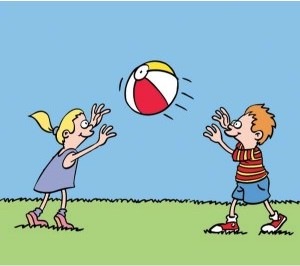
\includegraphics[width=0.25\columnwidth]{figures/I21.jpg}} \\
\hline
What is the girl doing? & What is the boy doing? & What is the boy doing? \\
\hline
\end{tabular}
%\caption{\label{tab:example-pdt-items} PDT example images with their targeted questions. In the untargeted form, the question for each is \textit{What is happening?} From left to right, the examples represent one intransitive, transitive and ditransitive item.}
\end{center}
\end{table}
\medskip
\end{frame}

\begin{frame}
\frametitle{Recap: Feature annotation}
\begin{table}[htb!]
\scriptsize
\begin{center}
%\begin{tabular}{|p{3.7cm}|c|c|c|c|c|}
\begin{tabular}{|l|c|c|c|c|c|}
\hline
\multicolumn{6}{|c|}{
\includegraphics[width=0.3\columnwidth]{figures/I02.jpg}} \\
\hline
\textit{What is the boy doing?} & C & A & G & I & V \\
\hline
\hline
He is eating food. & 0 & 1 & 1 & 1 & 1 \\
\hline
he eating. & 0 & 1 & 0 & 1 & 1 \\
\hline
The child is about to eat pizza. & 1 & 0 & 1 & 1 & 1 \\
\hline
He may get fat eating pizza. & 0 & 0 & 1 & 1 & 0 \\
\hline
\end{tabular}
\caption{\label{tab:dev-transitive} \scriptsize Annotated for five features: Core event (\textit{C}), Answerhood (\textit{A}), Grammaticality (\textit{G}), Interpretability (\textit{I}) and Verifiability (\textit{V}).}
\end{center}
\end{table}

\end{frame}

\begin{frame}
\frametitle{Recap: Feature annotation weights}
\scriptsize
I used a preference test to establish feature weights. In this toy example, weights are based on 3 pairs. The net score for the preferred responses for each feature is divided by the sum of all 5 net scores (sum$=$6; e.g., \textit{C} weight: 2/6$=$.333). The real weights$^*$ are based on 1200 pairs across all items.
\begin{table}
\scriptsize
\begin{center}
\begin{tabular}{|=l|+c||+c|+c|+c|+c|+c|}
\hline
\textit{What is the boy doing?} & Pref? & C & A & G & I & V \\
\hline
\multicolumn{7}{c}{} \\
\hline
\rowstyle{\color{OliveGreen}}He is eating food. & \textbf{yes} & \textbf{0} & \textbf{1} & \textbf{1} & \textbf{1} & \textbf{1} \\
\hline
\rowstyle{\color{Maroon}}He may get fat eating. & no & 0 & 0 & 1 & 1 & 0 \\
\hline
\multicolumn{7}{c}{} \\
\hline
\rowstyle{\color{Maroon}}He is hungry. & no & 0 & 0 & 1 & 0 & 1 \\
\hline
\rowstyle{\color{OliveGreen}}the boy is eating pizza & \textbf{yes} & \textbf{1} & \textbf{1} & \textbf{1} & \textbf{1} & \textbf{1} \\
\hline
\multicolumn{7}{c}{} \\
\hline
\rowstyle{\color{OliveGreen}}The child is about to eat pizza. & \textbf{yes} & \textbf{1} & \textbf{0} & \textbf{1} & \textbf{1} & \textbf{1} \\
\hline
\rowstyle{\color{Maroon}}he eating. & no & 0 & 1 & 0 & 1 & 1 \\
\hline
\multicolumn{7}{c}{} \\
\hline
\rowstyle{\color{OliveGreen}}Totals preferred responses & & 2 & 2 & 3 & 3 & 3 \\
\hline
\rowstyle{\color{Maroon}}Totals dispreferred responses & & 0 & 1 & 2 & 2 & 2 \\
\hline
\rowstyle{\color{OliveGreen}}Net preferred (pref {\color{black}-} {\color{Maroon}dispref}) & & 2 & 1 & 1 & 1 & 1 \\
\hline
Feature weight &  & .333 & .167 & .167 & .167 & .167 \\
\hline
\multicolumn{7}{c}{} \\
\hline
$^*$Real feature weight &  & .365 & .093 & .055 & .224 & .263 \\
\hline
\end{tabular}
%\caption{\label{tab:dev-transitive} \scriptsize Annotated for five features: Core event (\textit{C}), Verifiability (\textit{V}), Answerhood (\textit{A}), Interpretability (\textit{I}) and Grammaticality (\textit{G}).}
\end{center}
\end{table}

\end{frame}

\begin{frame}
\frametitle{Recap: Gold Standard}
\scriptsize
I applied the feature weights to the annotations to establish a gold standard (GS) score for each NNS response (n=70) for each PDT item. I ranked by GS score to get a GS ranking. (I use the real weights in this example.)
\begin{table}
\tiny
%\begin{table}[t!] This line is giving me trouble when I go to typeset
\begin{center}
%\begin{tabular}{|p{3.7cm}|c|c|c|c|c|}
\begin{tabular}{|l|l|c|c|c|c|c||l|c|}
%\hline
%\multicolumn{6}{|c|}{
\includegraphics[width=0.45\columnwidth]{figures/I02.jpg}} \\
%\multicolumn{6}{|c|}{
\includegraphics[width=0.3\columnwidth]{figures/I02.jpg}} \\
\hline
%\multicolumn{3}{|l|}{What is the woman doing? [Intransitive]} \\
Participant & \textit{What is the boy doing?} & C & A & G & I & V & \tiny{GS score} & \tiny{GS rank} \\
\hline
p1 & The boy is eating. & 0 & 1 & 1 & 1 & 1 & 0.635 & 4 \\
\hline
p2 & A baby is eating pizza & 0 & 0 & 1 & 1 & 0 & 0.279 & 5 \\
\hline
p3 & The boy enjoys his pizza. & 1 & 0 & 1 & 1 & 1 & 0.907 & 2 \\
\hline
p4 & the boy is eating pizza & 1 & 1 & 1 & 1 & 1 & 1.0 & 1 \\
\hline
p5 & The kid is eats pizza & 1 & 0 & 0 & 1 & 1 & 0.852 & 3 \\
\hline
\end{tabular}
%\caption{\label{tab:dev-transitive} \scriptsize Annotated for five features: Core event (\textit{C}), Verifiability (\textit{V}), Answerhood (\textit{A}), Interpretability (\textit{I}) and Grammaticality (\textit{G}).}
\end{center}
\end{table}

\end{frame}

\begin{frame}
\frametitle{Recap: Auto scoring}
\scriptsize
I have a system for automatically scoring the NNS responses. (The details aren't really important here, but ...)
\bigskip

For each item, the process is like this:

For the collection of NS responses  (n=50 per PDT item):

1) dependency parse;

2) get tf-idf score for each unique dependency (\textit{Compare against a large balanced corpus; common dependencies get low scores, rare dependencies get higher scores}).
\bigskip

For each NNS response, repeat \textit{1} and \textit{2}, then compare NS vs NNS (dependency scores vectors) -- use cosine. This is the NNS response score.

\bigskip

By selecting different parameters in this approach, I arrive at 12 different system configurations. Each configuration scores and ranks all NNS responses (n=70).

\end{frame}

\begin{frame}
\frametitle{Recap: Configurations}
\scriptsize

Rather than the full set of 12 configurations, let's consider this simplified set of 2 parameters $x$ 2 settings $=$ 4 configurations.
\medskip

\textbf{Parameters}:
\scriptsize
\begin{itemize}
\item \textbf{Dependency format}:
\begin{itemize}
\item \textbf{labeled}: e.g., nsubj(eat,boy); nobj(eat,pizza)
\item \textbf{unlabeled}: e.g., $\langle$null$\rangle$(eat,boy); $\langle$null$\rangle$(eat,pizza)
\end{itemize}
\item \textbf{NS response model}:
Each NS participant gave \textit{two} responses per PDT item
\begin{itemize}
\item \textbf{first}: Model contains only the first response from NS (n=50)
\item \textbf{mixed}: Model is half first reponses (n=25) and half second responses (n=25)
\end{itemize}
\end{itemize}
\begin{table}[htb!]
\scriptsize
\begin{center}
%\begin{tabular}{|p{3.7cm}|c|c|c|c|c|}
\begin{tabular}{|l|l|l|}
\hline
dep\textbackslash model & first & 1st \& mixed \\
\hline
labeled & lab\_first & lab\_mixed \\
\hline
unlabeled & unlab\_first & unlab\_mixed \\
\hline
\end{tabular}
\caption{\scriptsize Four system configurations for scoring NNS responses.}
\end{center}
\end{table}

\end{frame}


\begin{frame}
\frametitle{Recap: Gold Standard}
\scriptsize
I run the NNS responses through my system using the four different configurations. This yields a score and ranking for each response.
\begingroup
\setlength{\tabcolsep}{4pt} % Default value: 6pt
\begin{table}
\tiny
\begin{center}
\begin{tabular}{|l||c|c|c|c|c||l|c||l|c||l|c||l|c||l|c|}
\hline
P & C & A & G & I & V & \tiny{GS s} & \tiny{GS r} & \tiny{lf s} & \tiny{lf r} & \tiny{uf r} & \tiny{uf r} & \tiny{lm s} & \tiny{lm r} & \tiny{um r} & \tiny{um r} \\
\hline
p1 & 0 & 1 & 1 & 1 & 1 & 0.63 & 4 & .53 & 4 & .11 & 5 & 0.29 & 4 & .39 & 3 \\
\hline
p2 & 0 & 0 & 1 & 1 & 0 & 0.27 & 5 & .13 & 5 & .15 & 4 & 0.15 & 5 & .53 & 5 \\
\hline
p3 & 1 & 0 & 1 & 1 & 1 & 0.90 & 2 & .91 & 1 & .68 & 1 & 0.33 & 3 & .55 & 1 \\
\hline
p4 & 1 & 1 & 1 & 1 & 1 & 1.0 & 1 & .80 & 2 & .41 & 2 & 0.70 & 1 & .24 & 2 \\
\hline
p5 & 1 & 0 & 0 & 1 & 1 & 0.85 & 3 & .77 & 3 & .20 & 3 & 0.63 & 2 & .22 & 4 \\
\hline
\end{tabular}
\caption{\label{tab:modelranks} \scriptsize Response scores (\textit{s}) and ranks (\textit{r}) for: gold standard (\textit{GS}); four configurations: labeled\_first (\textit{lf}), unlabeled\_first (\textit{uf}), labeled\_mixed (\textit{lm}), unlabeled\_mixed (\textit{um}).}
\end{center}
\end{table}
\endgroup
\end{frame}

\begin{frame}
\frametitle{Stats questions}
\small
My goal at this point is to identify meaningful trends. I suspect that certain configurations or parameter settings will work better with particular kinds of items. Ideally, I could use such patterns to select the optimal configuration for intransitive items vs transitive items, etc.

\bigskip
\textbf{I need guidance how to approach this. Given my data, what analysis would you recommend?}

\bigskip
One caveat to note: the feature annotations are heavily skewed. For a handful of the (30 items $x$ 5 features $=$) 150 cases, a feature is ``1'' for \textit{all} 70 NNS responses.

\end{frame}


\begin{frame}
\frametitle{Stats questions}
\scriptsize
\medskip

I've tried experimenting with Spearman correlations to find trends.

\begingroup
\setlength{\tabcolsep}{5pt} % Default value: 6pt
\begin{table}
\tiny
\begin{center}
\begin{tabular}{|l||l|c||l|c||l|c|}
\hline
P & \tiny{GS s} & \tiny{GS r} & \tiny{lf s} & \tiny{lf r} & \tiny{uf r} & \tiny{uf r} \\
\hline
p1 & 0.63 & 4 & .53 & 4 & .11 & 5 \\
\hline
p2 & 0.27 & 5 & .13 & 5 & .15 & 4 \\
\hline
p3 & 0.90 & 2 & .91 & 1 & .68 & 1 \\
\hline
p4 & 1.0 & 1 & .80 & 2 & .41 & 2 \\
\hline
p5 & 0.85 & 3 & .77 & 3 & .20 & 3 \\
\hline
\hline
\multicolumn{3}{|l||}{Spearman $\rho$} & \multicolumn{2}{r||}{.899} & \multicolumn{2}{r|}{.799} \\
\hline
\multicolumn{3}{|l||}{Spearman p-val} & \multicolumn{2}{r||}{.037} & \multicolumn{2}{r|}{.104}  \\
\hline
\end{tabular}
\caption{\scriptsize \label{tab:spearman} By comparing the gold standard ranking (GS r) with a configuration ranking (e.g., lf r), I generate a Spearman correlation.}
\end{center}
\end{table}
\endgroup

\vspace{-4ex}
\begin{itemize}
\item 12 configurations $x$ 30 items $=$ 360 Spearman scores.
\item I used these scores to generate hierarchical clusters of items. I did this in nearly every conceivable way; I used: \textit{all} items; \textit{individual} items; I averaged Spearman scores for a given parameter setting, e.g., to compare labeled and unlabeled, I averaged \textit{labeled\_first} $+$ \textit{labeled\_mixed}, then averaged \textit{unlabeled\_first} $+$ \textit{unlabeled\_mixed}, then clustered items based on these two sets of values.
\item I hoped to find intransitive items clustered together, transitive items clustered together, etc. Any such trends appear very weak, however.

\end{itemize}

\end{frame}


\begin{frame}
\frametitle{Stats questions}
\scriptsize

Other ideas

\begin{itemize}

\item I've begun experimenting with \textbf{T-test} and \textbf{Wilcox} test. In this case, the idea is to analyze individual features. For example, for a given item and for a given configuration, group all responses where \textit{Core event} is annotated ``1'', then group all the ``0'' responses. Then run a \textbf{paired sample T-test} using the system score for those groups to see if there are significant differences between them. If I do this for all items, I can look for differences between the intransitive, transitive, ditransitive items across all configurations.

\item I'm also considering this approach but using \textbf{average precision} instead of T-test. In this case, I'd be looking for configurations that maximize the separation of ``0'' and ``1'' responses.

\item I believe 


\end{itemize}

\end{frame}


%\begin{beamercolorbox}{title}
%\mbox{}\\[1ex]%\vspace{1ex}
%\usebeamerfont{title}References
%\end{beamercolorbox}
%\medskip
%\scriptsize
%\bibliographystyle{styles/myaclnat}
%\bibliography{levi-bib}

\end{document}